\subsection{Interpretacion de los datos}

Recordemos que el objetivo principal del acceso a los datos, es obtener conocimiento. Hay que tener en 
cuenta que los datos por si solos, no tienen ningun valor, ya que carecen de sentido, una vez integrados en un contexto,
nos aportara informacion, y procesando y analizando esta informacion, se obtendra el conocimiento.\\
    
\begin{figure}[h]
    \centering 
    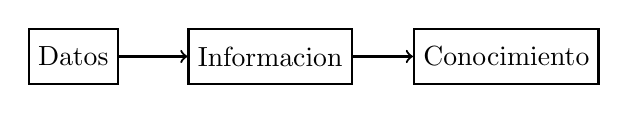
\begin{tikzpicture}[thick]
        \node[draw,rectangle,minimum size=20] (a) {Datos};
         \node[draw,rectangle,minimum size=20,right of= a, node distance=2.5cm] (b) {Informacion};
         \node[draw,rectangle,minimum size=20,right of=b, node distance=3cm] (c) {Conocimiento};
         \draw[->] (a) to (b);
        \draw[->] (b) to (c);
     
      \end{tikzpicture}
      \caption{Diagrama. De datos a conocimiento}
    \end{figure}
 
Para poder obtener este conocimiento de los datos, es necesario que el usuario interprete correctamente los datos, por lo
que el usuario debe contar con conocimientos en la materia o realizar una tarea de investigacion, que le permita 
entender los datos extraidos. \\

Asi pues, para que el usuario pueda obtener la informacion de una manera directa, requiere de conocimientos tanto 
de programacion como especificos de la materia y los recursos para crear una infraestructura que le permita implementar 
una representacion de los datos que le sea util.\\

Podemos concluir que el acceso a los datos por parte del usuario medio, no es directa.\\

Para poder construir un sistema que haga los datos accesibles, es imprescindible disenar un modelo  para concretar la 
informacion que se desea obtener. El diseno de un sistema permitira que a partir de unos valores dados, proporcione unos resultados.
Para ello sera necesario tener un conocimiento solido del conjunto de datos que se necesita, los valores,
sus unidades y como se relacionan entre si.\\


\noindent\textbf{\textit{Aire Guru} }\\


Aire Guru se ocupa de representar el EAQI (European Air Quality Index) general calculado sobre un mapa. Este es un formato mas legible para los usuarios.
Este indice mustra un indicador con cinco niveles: "Insalubre" "Malo" "Pobre" "Aceptable" y "Bueno" y especifica un rango de colores desde el rojo hasta el celeste.

\begin{figure}[ht]
    \centering
    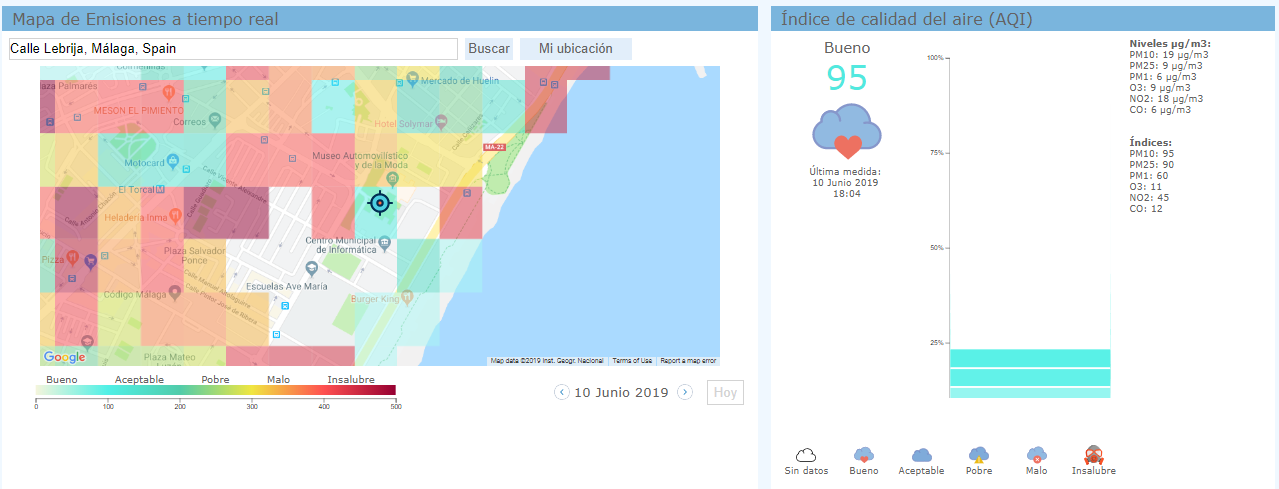
\includegraphics[width=12cm]{mapAireGuru}
    \caption{Aire Guru. Landing page. Top section}
\end{figure}
Nuestra plataforma introduce ademas una iconografica para ayudar al usuario a tener una idea directa de la situacion, ya que son mas 
explicativos que los colores. En caso de peligro, queda bien representado con el color rojo, pero en el caso del azul o verde, en nuestra cultura, no
tenemos definido un estado para estos colores.
\begin{figure}[ht]
    \centering
    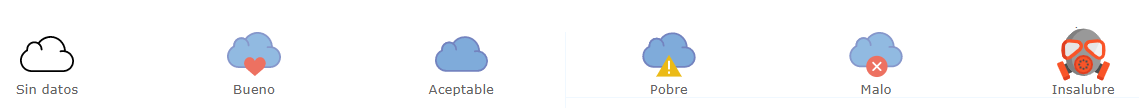
\includegraphics[width=12cm]{EAQUI_Icons}
    \caption{Iconografica Aire Guru}
\end{figure}
\newpage
\begin{itemize}
    \item \textit{Evaluation}
\end{itemize}
